\documentclass{beamer}
\usepackage{graphicx}
\usepackage{paralist}
\usepackage{outlines}

\title{Brush and Pencil Tools}
\author{Mendocino College - DAM 110}
\titlegraphic{\vspace{-10mm}
\includegraphics[width = .8\textwidth]{images/photoshop.jpg}} 
\date{\vspace{-5em}} 


\mode <presentation>
\usetheme{Warsaw}
\usecolortheme{default}

\setbeamerfont{footline}{size=\fontsize{5}{8}\selectfont}

\definecolor{darkred}{rgb}{20,0,0}
\definecolor{darkgreen}{RGB}{40,110,20}
\definecolor{darkpurple}{RGB}{30,0,30}
\definecolor{chardonnay}{RGB}{255, 255, 204}

\setbeamercolor*{palette primary}{fg=white, bg=darkgreen}


\begin{document}
	{
		\setbeamertemplate{footline}{} 
		\setbeamertemplate{headline}{} 
		\begin{frame}
			\vspace{-35pt}
			\maketitle
		\end{frame}
	}



	\section{The Painting Tools}
		\begin{frame}
		\frametitle{The Painting Tools}
		\begin{center}
			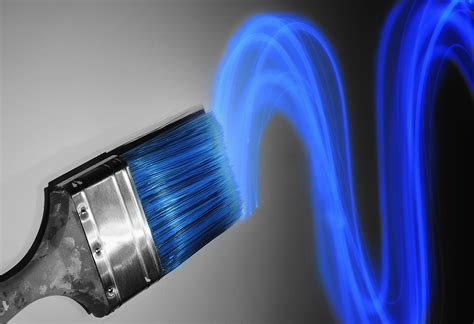
\includegraphics[width = 0.8\textwidth]{images/brush.jpg}
		\end{center}
	\end{frame}
	
			\subsection{What are the Painting Tools?}		
	\begin{frame}
		\frametitle{What are the Painting Tools?}
	\begin{outline}
		\1 The Brush tool and the Pencil tool work like traditional drawing tools applying color with brush strokes.
		\1 The Brush tool and the Pencil tool paint the current foreground color on an image. 
	\end{outline}
\begin{center}
	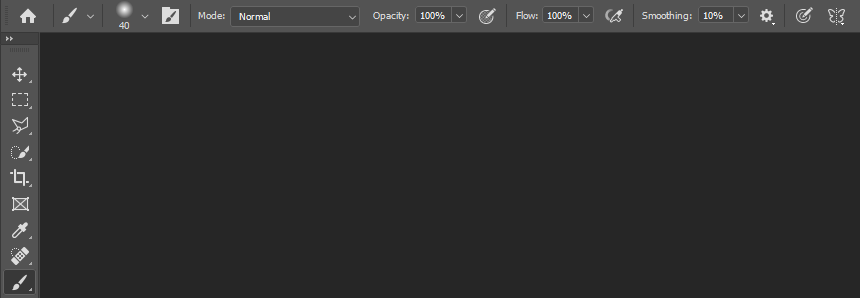
\includegraphics[width=1.0\textwidth]{images/brush tool.png}
\end{center}
		\end{frame}
	
			\subsection{What is the Brush Tool?}		
\begin{frame}
	\frametitle{What is the Brush Tool?}
	\begin{outline}
		\1 It creates soft strokes of color.
		\1 It works by adding a shaped mark on a layer
	\end{outline}
	\begin{center}
		
\includegraphics[width=.7\textwidth]{images/brush.png}
	\end{center}
\end{frame}

			\subsection{What is the Pencil Tool?}		
\begin{frame}
	\frametitle{What is the Pencil Tool?}
	\begin{outline}
		\1 It creates hard strokes of color.
		\1 It works by adding a shaped mark on a layer
	\end{outline}
		\begin{center}
	
\includegraphics[width = 1.0\textwidth]{images/Pencil-Tool-in-Photoshop.jpg}
\end{center}
\end{frame}




\subsection{The Basics}
\begin{frame}
		\frametitle{The Basics}

	\begin{outline}
		\1 Click the little arrow in-between the brush example and folder with a brush on it.
		\1 Size
		\2 Increases or decreases the size of the brush tip.
		\2 Brackets are the Keyboard Shortcuts to increase/decrease Size
		\3 $$\left[ and \right]$$
		\1 Hardness
		\2 Increases or decreases the brush tip's border strength.
		\2 0\% means a soft border, and 100\% a precise border. 
	\end{outline}
\begin{center}
	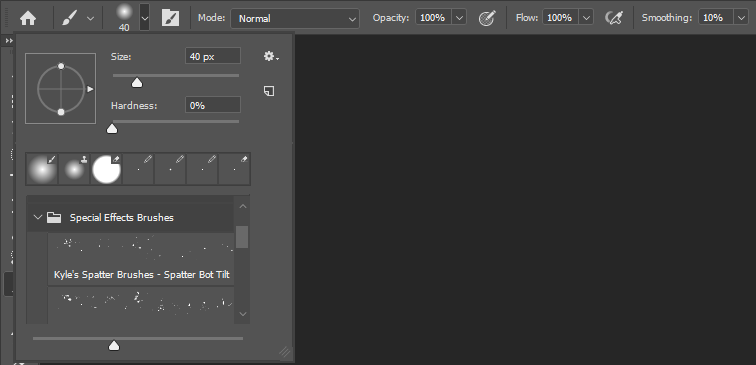
\includegraphics[width=.7\textwidth]{images/brush tool basics.png}
	\end{center}
\end{frame}

\subsection{Choosing Colours}
\begin{frame}
	\frametitle{Choosing Colours}
	\begin{outline}
		\1 The color being applied by the brush tip is controlled by the Foreground Color, found at the bottom of the Tools toolbar. 
		\1 To change the brush color in Photoshop, click on the Foreground Color and use the Color Picker to choose a new color. 
	\end{outline}
	\begin{center}
		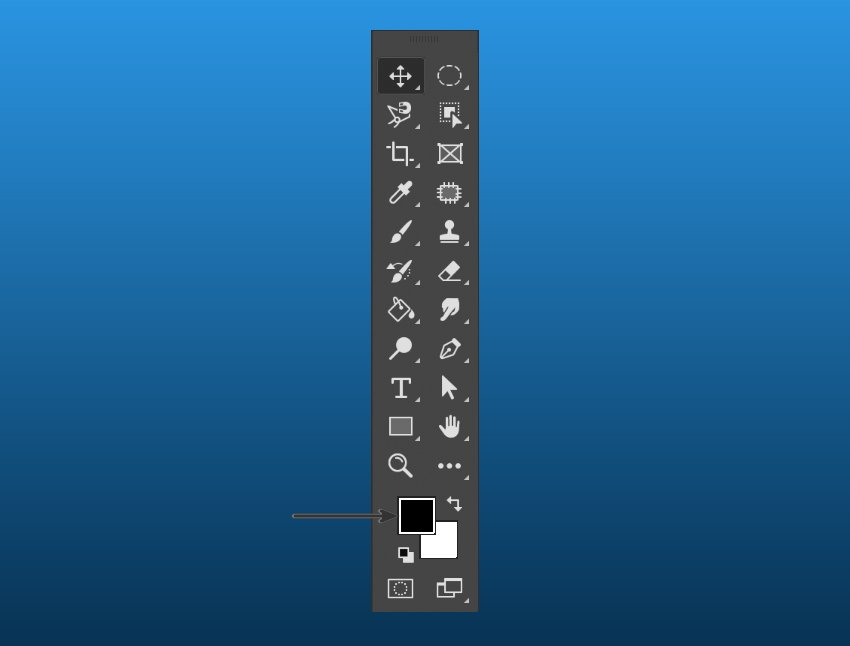
\includegraphics[width = 0.6\textwidth]{images/2.2.jpg}
	\end{center}
\end{frame}


\section{Brush Tips}	
\subsection{Brush Tips}	
\begin{frame}
	\frametitle{Brush Tips}
	\begin{outline}
		\1 Lets you change the shape you are drawing with.
	\end{outline}
	\begin{center}
		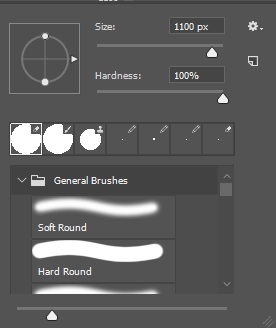
\includegraphics[width = 0.6\textwidth]{images/brush tips.png}
	\end{center}
\end{frame}

\section{Brush Modes}	


\subsection{Opacity}	
\begin{frame}
	\frametitle{Opacity}
	\begin{outline}
		\1 The Opacity value is a percentage of transparency 
		\2 100\% means a full-color stroke, while a smaller percentage indicates a more transparent stroke.
	\end{outline}
	\begin{center}
		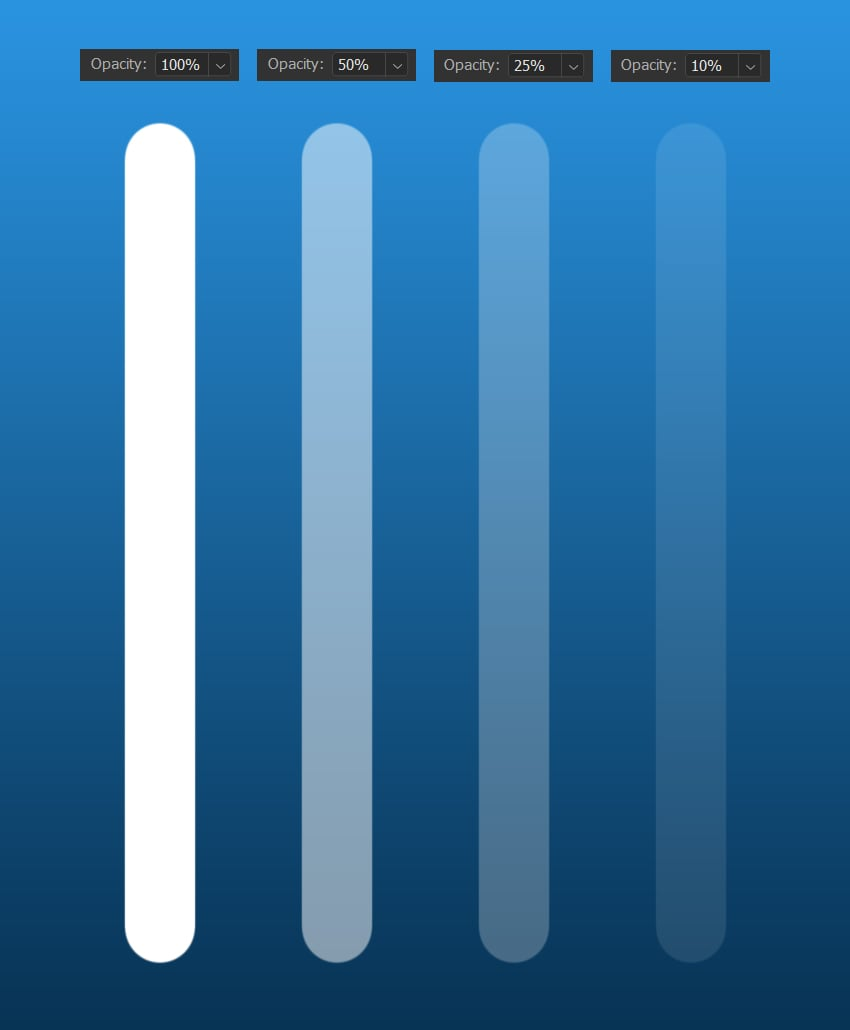
\includegraphics[width = 1.0\textwidth]{images/2.6.jpg}
	\end{center}
\end{frame}

\subsection{Flow}	
\begin{frame}
	\frametitle{Flow}
	\begin{outline}
		\1 The Flow setting controls the speed at which paint is laid down. 
		\1 Each pass of the brush over the same spot will build more and more paint. 
		\2 Unlike with Opacity, you don’t have to lift your brush, making it ideal for gradually building up things like color, light, and shadows!
	\end{outline}
	\begin{center}
		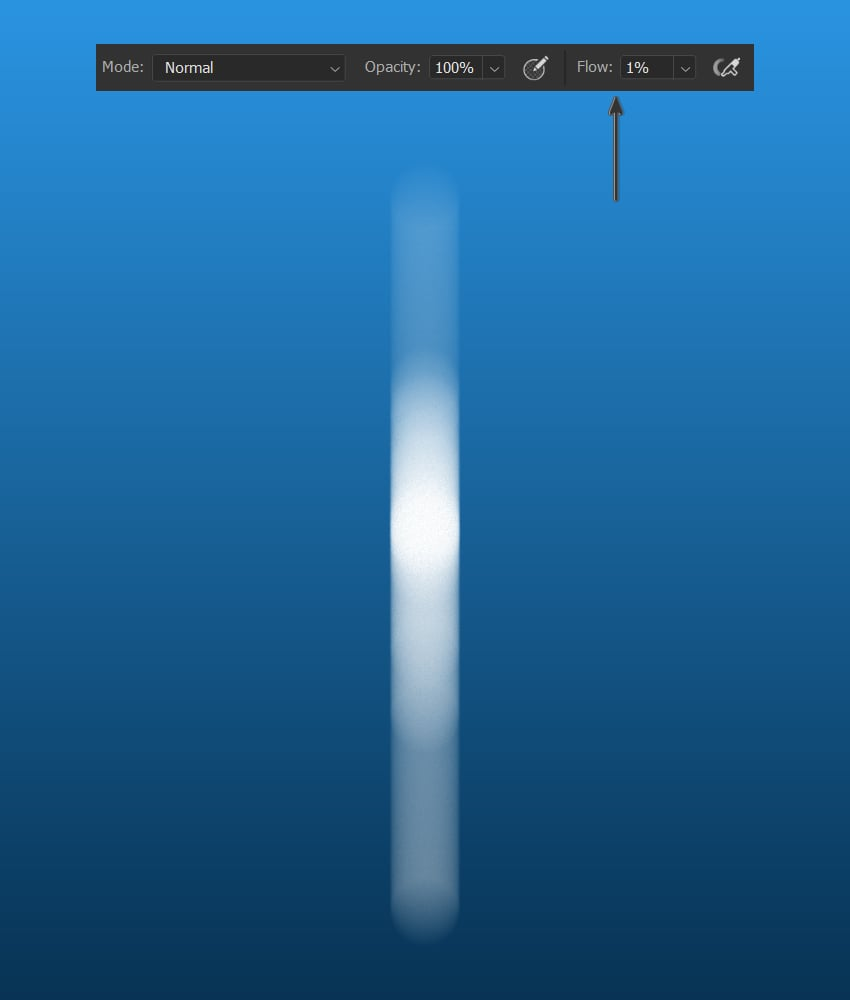
\includegraphics[width = 0.6\textwidth]{images/2.7.jpg}
	\end{center}
\end{frame}

\subsection{Smoothing}	
\begin{frame}
	\frametitle{Smoothing}
	\begin{outline}
		\1 Photoshop performs intelligent smoothing on your brush strokes.
		\1 A value of 0 is the same as legacy smoothing in earlier versions of Photoshop. 
		\2 Higher values apply increasing amounts of intelligent smoothing to your strokes.
		\1 Enter a value (0-100) for Smoothing in the Options bar when you're working with one of the following tools: Brush, Pencil, Mixer Brush, or Eraser. 
	\end{outline}
	\begin{center}
		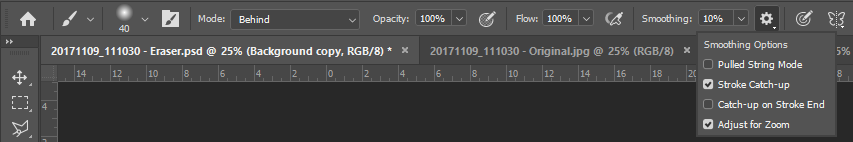
\includegraphics[width = 1.0\textwidth]{images/smoothing.png}
	\end{center}
\end{frame}

\begin{frame}
	\frametitle{Smoothing Options}
	\begin{outline}
		\1 Stroke smoothing works in several modes. Clicking the gear icon to enable one or more of the following modes:
		\1 Pulled String Mode
		\2 Paints only when the string is taut. Cursor movements within the smoothing radius leave no mark.
		\1 Stroke Catch Up
		\2 Allows the paint to continue catching up with your cursor while you've paused the stroke. Disabling this mode stops paint application as soon as the cursor movement stops.
		\1 Catch-Up On Stroke End
		\2 Completes the stroke from the last paint position to the point where you released the mouse/stylus control.
		\1 Adjust For Zoom
		\2 Prevents jittery strokes by adjusting smoothing. Decreases smoothing when you zoom in the document; increases smoothing when you zoom out.
	\end{outline}
\end{frame}

\subsection{Blending Modes}	
\begin{frame}
	\frametitle{Blending Modes}
	\begin{outline}
		\1 Sets the method for blending the color you paint with the underlying existing pixels.
		\1 Each time you paint something using the Brush Tool, you can choose a Blending Mode for the stroke. 
		\1 A Blending Mode is a way to change how a brushstroke interacts with the pixels behind the stroke. 
	\end{outline}
	\begin{center}
		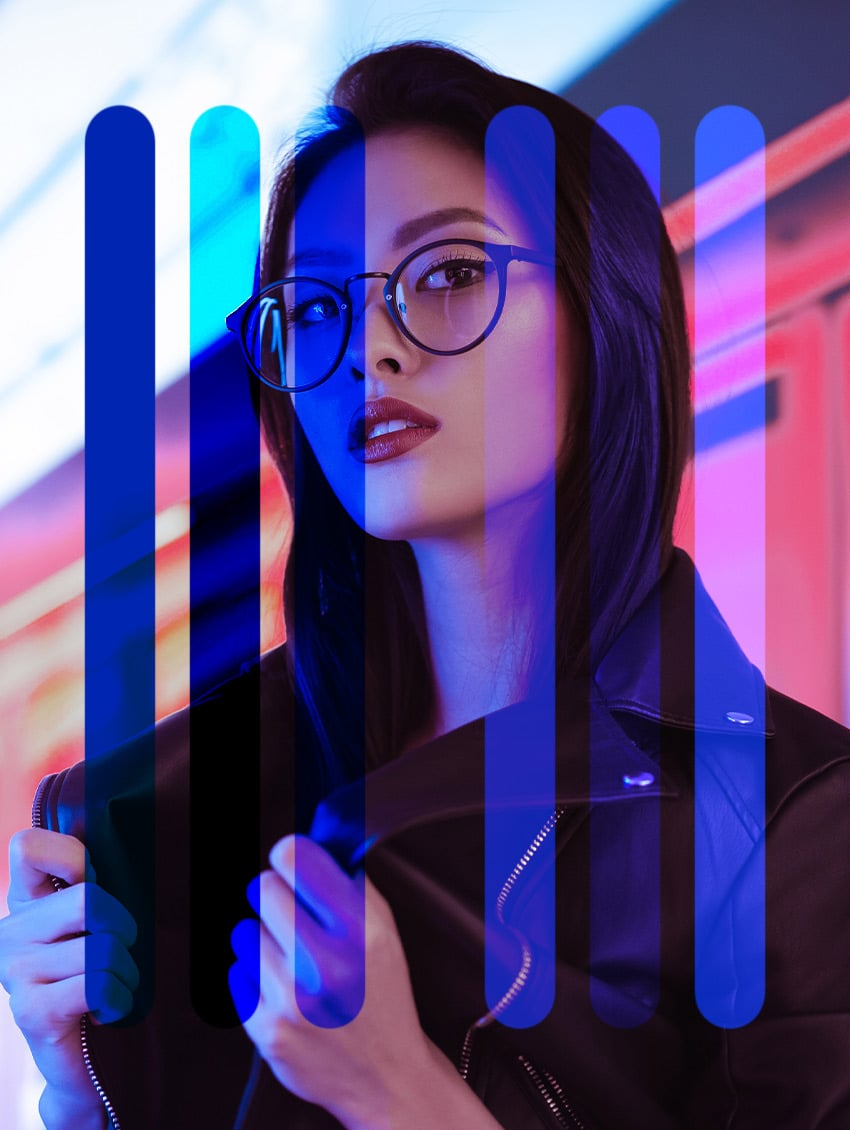
\includegraphics[width = 0.4\textwidth]{images/2.5.jpg}
	\end{center}
\end{frame}

\begin{frame}
	\frametitle{Example Blending Modes}
	\begin{outline}
		\1 The first on the list is Normal Mode, which paints the color as is. 
		\1 The Second is Dissolve Mode adds some noise at the edge of the brush stroke.
		\1 The Third is Behind Mode which paints behind an existing stroke, even if they are both on the same layer.
		\1 And then Clear Mode. The “Clear” blend mode turns the pixels you paint on transparent, much like the Eraser tool.
	\end{outline}
	\begin{center}
		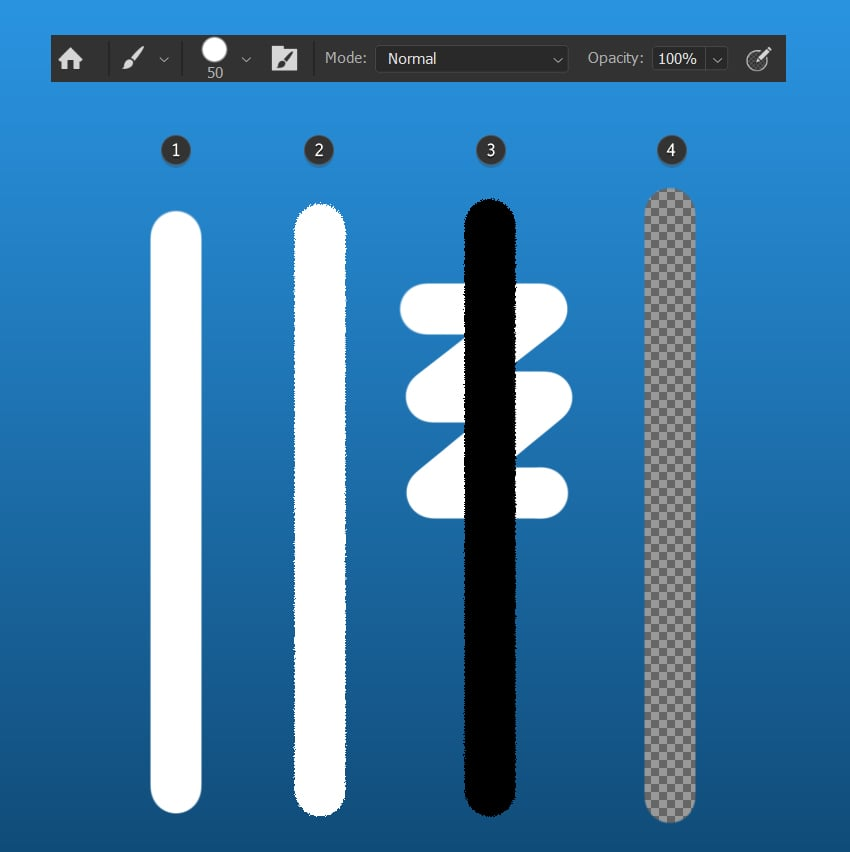
\includegraphics[width = 0.5\textwidth]{images/2.4.jpg}
	\end{center}
\end{frame}

\section{Brush Settings}	
\subsection{Brush Settings}	
\begin{frame}
	\frametitle{Brush Settings}
		\begin{columns}
		\column{.6\textwidth}
		\vspace{-15pt}
		\begin{itemize}
			\item The place to create, edit, save, and load a particular brush behavior or Brush Presets
			\item You can customize several things here like the brush tip shape, scattering, opacity jitter, flow jitter, configure controls for each variation, and more
			\item To show the Brush Settings Panel, in the Menu Bar go to Window then Brush Settings.
			\item Or Press F5 to show/hide the Settings Panel
		\end{itemize}
		\column{.45\textwidth}
		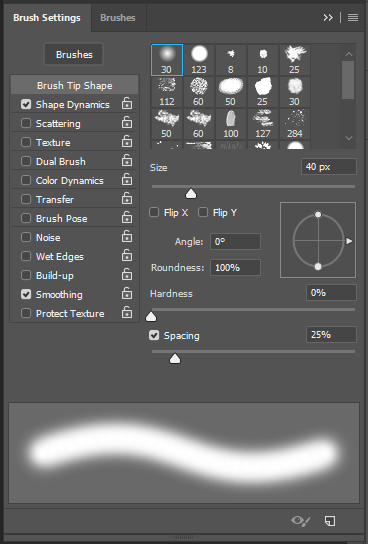
\includegraphics[width = 1.0\textwidth]{images/brush settings.png}
	\end{columns}
\end{frame}
	

\end{document}